\section{Paragraf autorstwa Krzysztof Baumgart}
\begin{flushleft}
    \textbf{Piece wędzarnicze.}
    
    \Large {Piece wędzarnicze są to urządzenia do przeprowadzania obróbki żywności w umiarkowanych temperaturach przy dużym zadymieniu pochodzenia organicznego.}
   
\begin{figure}[ht!]
\centering
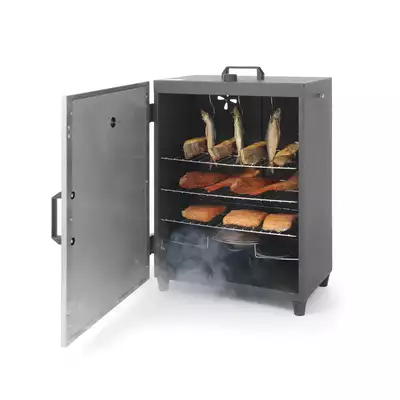
\includegraphics[width=90mm]{pictures/piec.jpg}
\caption{Piec wędzarniczy. \label{overflow}}
\end{figure}
    
    Wędzenie jest procesem, w trakcie którego przetwory poddawane są działaniu ciepła i związków chemicznych zawartych w dymie wędzarniczym. Dym otrzymywany jest w wyniku spalania odpowiedniego drewna i jego pochodnych (zręby i trociny wędzarnicze). W wyniku wędzenia następuje zmniejszenie zawartości wody w produkcie, a także zmiany chemiczne i fizykochemiczne. 
    
    Tradycyjne wędzenie spełnia dwa zasadnicze zadania:
    
    
    
\end{flushleft}